% This is a general template file for the LaTeX package SVJour3
% for Springer journals. Original by Springer Heidelberg, 2010/09/16
%
% Use it as the basis for your article. Delete % signs as needed.
%
% This template includes a few options for different layouts and
% content for various journals. Please consult a previous issue of
% your journal as needed.
%
\RequirePackage{fix-cm}
\documentclass{amsart}       
\usepackage{graphicx,tikz, fdsymbol}
\usepackage{bm,mathtools,setspace}% bold math
\usepackage[marginratio=1:1,textwidth=6in, textheight=8.5in]{geometry}
\usepackage[sort, authoryear, round]{natbib} % bibliography

\doublespacing
\begin{document}

\title{}
\author{Mohammad A. Khan        \and
        Rob Stoll %etc.
}

\maketitle

\begin{abstract} 
Previous studies confirmed the presence of Very Large Scale Motions (VLSMs) in channel and ABL flows through experimentation and simulations. However, due to limitations in experimentation and the lack of the account of Coriolis force in numerical simulations, the effects of rotation on VLSM have not been thoroughly examined.  Here, the Large Eddy Simulation technique was used to simulate VLSMs under different degrees of rotation.  Both traditional statistical and image processing  techniques were than used to characterize them. The traditional method of determination of length scales of VLSMs from per-multiplied spectra of the stream-wise velocity component proved to be inadequate when rotation was introduced. By identifying the footprints of VLSMs as connected regions of low momentum fluid and then identifying those regions through standard image processing tools, the difficulties in determining  the VLSM length scales could be circumvented. It was found that rotation inhibited the coherence and suppressed the development of VLSMs in the ABL flows. Also, it was found that the usual practice of visually identifying  VLSM on numerically filtered velocity fields as long regions of low momentum might not be sufficiently accurate.  

%Include keywords, PACS and mathematical
%subject classification numbers as needed.
%\keywords{ Atmospheric Boundary Layer  \and Coriolis Force  \and Large Eddy Simulation \and Very Large Scale Motion}
% \PACS{PACS code1 \and PACS code2 \and more}
% \subclass{MSC code1 \and MSC code2 \and more}
\end{abstract}

\section{Introduction}
\label{intro} 
%need to add in  ref to Chinhaka and Anderson 2017 (already in bib file)
In general turbulent flows  are composed of constituent coherent structures and background flows \citep{hussain_1986_jfm} and the dynamics and role of coherent structures are fundamental to the understanding of complex motions and mixing processes in the Atmospheric Boundary Layer (ABL) \citep{lewalle_flowTurbCom_00,Fiedler_PAeroSci_1988}. Recently, Very Large Scale Motions (VLSMs) in the ABL have garnered significant interests \citep[eg.][]{Chinthaka_blm_2017,kerherv_roux_etfs_2017}. VLSMs  are identified as  very long regions of low-momentum fluid aligned in the streamwise direction that are flanked by high-momentum regions and they have been observed in turbulent pipe \citep{guala_adrian_jfm2006, kim_adrian_pof99, monty_jfm_07}, channel \citep{guala_adrian_jfm2006, monty_jfm_07, lee_sung_jfm_14} and boundary layer flows \citep{fang2015blm,hutchins_marusic_jfm2007}. The rich features of VLSMs and their importance were demonstrated in both experimental \citep{kim_adrian_pof99,guala_adrian_jfm2006,hutchins_marusic_jfm2007,monty_jfm_07} and numerical studies \citep{fang2015blm,lee_sung_jfm_14,Lee_sung_jfm11}. However, a concrete definition of VLSMs is lacking which makes the identification of these structures highly subjective. A threshold value has to be chosen to differentiate between the low momentum streaks and the bulk flow and it has been shown that the chosen threshold value dictates the number of VLSMs detected for a particular length scale on a given horizontal plane \citep{baltzer_jfm_13}. In all of these applications, the length scale of VLSMs scales with $\delta$ where, $\delta$ refers to Boundary Layer (BL)  height, channel half width or pipe radius \citep{chung_jfm_10_large,monty_jfm_07}. From flow visualizations, the largest length scale of VLSMs was shown to be approximately $20\delta$. However, from two-point correlation the length scale is consistently under predicted and was reported to vary from $2.5\delta$ to $4\delta$ in the outer region of the BL. \citet{hutchins_marusic_jfm2007} hypothesized that the spanwise meandering of VLSMs could be responsible for the underestimation of streamwise length scales from two-point correlations of streamwise velocity. In this context another important length scale has been identified to be important which is smaller than VLSMs but plays dynamically important role like VLSMs. Structures corresponding to these length scale have been termed as the Large Scale Motions (LSMs). The presence of VLSMs causes a secondary peak to appear in the large wavelength region of the pre-multiplied spectra. While the streamwise autocorrelation has been found to be insufficient at identifying VLSM streamwise length scales, pre-multiplied spectra has been observed to be of the same the order or magnitude compared to  visualization of instantaneous flow fields \citep{guala_adrian_jfm2006}. In the spanwise direction the extent of VLSMs has been observed to be nearly an order of magnitude  smaller than the  streamwise length scale \citep{monty_jfm_07}. 

The importance of VLSMs manifest in their  contribution to the overall magnitude of Reynold's stress and turbulent kinetic  energy.  A cumulative  distribution  of turbulent kinetic energy  and Reynold's stress  over Fourier modes revealed that in pipe flow  more than $65\%$ of turbulent energy was due to very large scale motions while their contribution to Reynold's shear stress accounted as much as $60\%$ \citep{guala_adrian_jfm2006}. It was also found that large scale motions with an estimated eddy turn over time of $2\delta/U_{\infty}$ (where, $U_{\infty}$ denotes the free streamwise velocity) or greater strongly modulate the magnitude of smaller scale fluctuations within the log region and they modulate the frequency of small scale fluctuations even more significantly above the log region \citep{ganapathi_jfm_2012_modulation}. 


Here, our focus is the characterization of VLSMs in the ABL and how they are impacted by the Coriolis force. Unlike small scale laboratory flows, the effect of the earth's rotation can not be ignored in the ABL and to faithfully represent the physics, conservation equations must be studied in a rotational frame of reference.  When conservation of momentum is expressed in a rotational frame, the earth's rotation is accounted for by the introduction of a Coriolis force which can have an impact on the size and shape of the large eddies in the flow field \citep{esau_jot_2002}. The Coriolis force is often referred to as a fictitious force due to lack of contribution to the velocity magnitude and eventually to the mean kinetic energy or turbulent kinetic energy (TKE). Its importance in kinetic energy redistribution among different scales can be identified in case of low Rossby number ($Ro$) \citep{yeung_zhou_pof_98,hossain_pof_94}. In the limiting case of zero, $Ro=0$  i.e. in case of solid body rotation or low enough $Ro$ number where inertia is negligible compared to Coriolis force Taylor Proudman column of vortices are observed. It is the Ro number that signifies the  importance of a rotational frame of reference and defined as,  $Ro=\frac{U}{2\Omega L}$, where $U$ is the characteristic flow velocity usually a velocity associated with the integral length scale, $\Omega$ is the rate of rotation of the reference frame and $L$ is the characteristic length scale of the flow usually taken as the integral length scale.   It can  intuitively be predicted that Coriolis force  can have an impact on large scale coherent structures although, the effect is not readily comprehensible.   

% \citet{bourouiba_straub_jfm11} analyzed  energy transfer from 3D inertial wave vector modes ($k_x \hat{i}+k_y \hat{j} + k_z \hat{k}$ ) to vortical zero frequency modes ($k_x \hat{i}+k_y \hat{j}$) in forced rotating turbulence in the $1.5-8\times 10^{-2}$ Ro number regime and concluded that energy transfer between the aforementioned wave vector modes is responsible for emergence of columnar structures \citep{bourouiba_straub_jfm11}.

% Most of the above paragraph should be moved to after the VSLM description.
 
A consistent theme in VLSM studies is the identification and analysis of their spatial structure and evolution. Previous studies found that organized  VLSMs show the presence of finer scales and that the spatial development of VLSMs occur mainly as a result of the merger of smaller scale motions \citep{Lee_sung_jfm11,baltzer_jfm_13,lee_sung_jfm_14}. One of the possible mechanisms for the development of VLSMs is the merger of  hairpin packets marching forward in the downstream direction \citep{Lee_sung_jfm11}. Another possible  explanation is that concatenation of fast moving upstream LSMs with slow moving downstream LSMs constitute VLSMs \citep{lee_sung_jfm_14}. In the same study, it was also speculated that streamwise-elongated inclined hairpin vortex packets induce negative streamwise fluctuations that manifest as long-low momentum streaks in the streamwise direction \citep{lee_sung_jfm_14}. The association of counter rotating vortex rolls with VLSMs has also been reported as identified from Large Eddy Simulation (LES) \citep{fang2015blm}.  These  mechanisms of VLSM formation while offering a qualitative description, do not provide a comprehensive definition of the VLSMs and their evolution.
 
The main objective of this study is to discern the effect of rotation on the characteristics of VLSMs.  LESs were carried out over large domains to simulate the Earth's rotational effect.  We focused on the coherence of the flow and looked into the  known  signatures of VLSMs to understand how rotation impacts their characteristics.  The quantitative aspect of the contribution of VLSMs under the effect of rotation  in overall energy content, and  Reynold's stresses were studied.  A relatively straight forward  definition of VLSMs was developed to facilitate a VLSM detection method based on widely used image processing techniques. 

\section{Numerical Simulation}
%this section needs to be rearranged into a more coherent form.  First describing the general methodology, then the specific setup.  The horizontal mean profiles should be a different section.
In this study, LES technique was used examine the effect of rotation on very large scale motions.  The models and numerics used in the simulation code are described in detail in \citet{stoll_wrr_2006} and \citet{stoll_blm_2008}.  Here only a brief summary is given.  The numerical code solves the spatially filtered incompressible Navier-Stokes equations in rotational form,
\begin{equation}
    \frac{\partial \tilde{u}_i}{\partial t}+ \tilde{u}_j\left(\frac{\partial \tilde{u}_i}{\partial x_{j}} -\frac{\partial \tilde{u}_j}{\partial x_{i}} \right)  = -\frac{\partial \tilde{p^*}}{\partial x_i}-\frac{\partial \tau_{ij}}{\partial x_j}+f_{c}\epsilon_{ij3}\tilde{u}_{j},  
\label{eqn:les_eqn}
\end{equation}
\noindent where $\tilde{u}_i$ denotes the spatially filtered, resolved velocity in the $i-th$ direction, $p^{*}=p'/\rho + \frac{1}{2}\tilde{u}_i\tilde{u}_i$ is the modified pressure, $\tau_{ij}$ is the subgrid scale (SGS) stress tensor, and $f_c$ is the Coriolis parameter with a prescribed value of $10^{-4}\ s^{-1}$.  Viscous forces were assumed to be negligible as a result of the extremely high Reynolds number of the ABL and $\tau_{ij}$ was computed using the scale dependent Lagrangian-averaged dynamic Smagornisky model of \citet{stoll_wrr_2006}. Horizontal derivatives were calculated using a pseudo spectral method while, vertical derivatives were approximated using second-order central differences, and for time integration the second-order Adams-Bashforth scheme was used. As surface boundary conditions, the required instantaneous surface shear stresses $\tau_{i3,s}(x,y,t)$  were computed from the instantaneous filtered velocity field at the lowest vertical grid level by local application of the Monin-Obukhov similarity theory \citep{stoll_blm_2006} as:
\begin{align}
\tau_{i3,s}(x,y,t) = -\left [ \frac{\tilde{u}_r(x,y,z,t)\kappa}{\ln(z/z_o)} \right ]^2\frac{\tilde{u}_i(x,y,z,t)}{\tilde{u}_r(x,y,z,t)}, 
\end{align}
\noindent where, $\kappa$ is the von karman constant ($=0.4$), $z_o$ is the local aerodynamic roughness (= 0.1m in all simulated cases), and $\tilde{u}_r(x,y,z,t)=[\tilde{u}_1(x,y,z,t)^{2}+\tilde{u}_2(x,y,z,t)^{2}]^{1/2}$ is the local horizontal wind speed. Although application of Monin-Obukhov similarity theory is not strictly valid instantaneously and locally, sensitivity tests indicate that its primary impact on the flow dynamics is confined to the lowest computational levels \citep{stoll_blm_2006}. This numerical code has also been used to simulate the ABL under a variety of different forcing conditions \citep[e.g.,][]{stoll_jas_2009,bailey_blm_2013,miller_blm_2013} and to examine the structure and evolution of turbulent motions \citep[e.g.,][]{bailey_ae_2014,bailey_jfm_2016}.  Its excellent representation of SGS momentum fluxes \citep{stoll_wrr_2006} makes it ideal for an examination of large-scale ABL velocity field dynamics.

% The lateral boundary conditions were assumed to be periodic.  In all simulations, a zero stress condition was used at the top domain boundary i.e. $\partial\tilde{u}_1/\partial x_3 = \partial \tilde{u}_2/\partial x_3=0$.

\subsection{Simulation Setup}
Three different simulated flow cases designated as $CHNL$, $EK10$, and $EK02$ were examined to assess the effect of rotation on the characteristics of VLSMs in the ABL. Each case was characterized by a different $Ro$ with $CHNL$ a classical channel flow simulation under neutral stability condition driven by a constant horizontal pressure  gradient, and $EK10$ and $EK02$ are Ekman layer simulations under different degrees of rotation induced by geostrophic velocities. The $CHNL$ case can be considered as a limiting case with an infinite $Ro$. 


The focus of the study is large scale dynamics and therefore, the simulation domain spans large horizontal extents in streamwise ($L_{x}=128\ Km$) and spanwise ($L_{y}=128\ Km$) directions and has a height of $1500\ m (L_z)$ for $CHNL$ and $EK10$ and a height of $750\ m$ for $EK02$ in the vertical direction. The corresponding numerical grid is discretized with $N_{x}= 2048$, $N_{y}=2048$ and $N_{z}=64$ nodes. A summary of the discretization along with basic parameters of the simulations are furnished in table \ref{tab:sim_param} where, $u_*$ denotes the friction velocity, $U_g$ denotes the geostrophic wind velocity in the x-direction (streamwise) and $\delta$ stands for the boundary layer height, and $f$ is the Coriolis parameter.
For the $CHNL$ case the flow is driven by a constant mean pressure gradient along the streamwise direction with a prescribed value of $\left < \rho^{-1} \frac{\partial \tilde{p}}{\partial x} \right > = 1.3419\times 10^{-9}\ ms^{-2}$ where, $\left <  \right >$ denotes a horizontal mean. The last term in Eqn. \ref{eqn:les_eqn} is absent for $CHNL$ because there is no rotation of the reference frame. Stress free ($\frac{\partial \tilde{u}_1}{\partial z}=\frac{\partial \tilde{u}_2}{\partial z}=0$) conditions are imposed at the top of the domain. Initially, a logarithmic mean vertical velocity profile typical of channel flows is generated resulting in a velocity of $10\ ms^{-1}$ at a height of $L_z$, and a perturbation with a magnitude of  $0.25 u_*^{2}$ is added to the velocity components ($u_1,\ u_2,\ u_3$) in the logarithmic layer. For the $EK10$ and $EK02$ cases geostrophic wind velocities ($U_{g}$) of $10\ ms^{-1}$ and $2\ ms^{-1}$ are specified, respectively. At the top of the boundary the assumed balance between pressure and Coriolis force ($\left < \rho^{-1}\frac{\partial \tilde{p} }{\partial x_i} \right > = f_c\epsilon_{ij3}\tilde{u}_j$) and the imposed stress free condition ($\frac{\partial \tilde{u}_1}{\partial z}=\frac{\partial \tilde{u}_2}{\partial z}=0$) result in the formation of an Ekman layer. Consequently,  the mean pressure gradient that sustains the flow does not change in the wall-normal direction, throughout the BL.  In terms of forcing the difference between the simulated $CHNL$ and Ekman layer simulations is that, in $CHNL$ a constant $\left < \rho^{-1} \frac{\partial \tilde{p}}{\partial x} \right >$ acts on the flow while in $EK10$ and $EK02$ a constant $\left < \rho^{-1}\frac{\partial P }{\partial y} \right >  = -f_c U_g$ is forcing the flow. Precursor simulations were carried out to generate initial flow fields for $EK10$ and $EK02$ using a one dimensional single column model following the initialization procedure of \citet{andren_brown_qjrm_94}. Prognostic equations for the precursor simulations of $EK10$ and $EK02$ are shown in equation \ref{eqn:prognostic_precursor}.
\begin{align}
\frac{\partial \left < u_{1} \right >}{\partial t}=f(\left < u_{2} \right > - V_g)-\frac{\partial }{\partial z}(u_{1}'u_{3}') \notag \\
\frac{\partial \left < u_{2} \right > }{\partial t}=f(\left < u_{1} \right > - U_g)-\frac{\partial }{\partial z}(u_{2}'u_{3}').
\label{eqn:prognostic_precursor}
\end{align} 
The turbulent stresses in eq. \ref{eqn:prognostic_precursor} $\left < u_{1}'u_{3}' \right >$ and $\left < u_{2}'u_{3}' \right >$ are estimated using eddy diffusivity models, $\left < u_{1}'u_{3}' \right > = -k_{m}^{u}\frac{\partial \left < u \right >}{\partial z}$ and $\left < u_{2}'u_{3}' \right > =-k_m^{v}\frac{\partial \left < v \right >}{\partial z}$. Eddy diffusivities in turn were approximated using a single equation mixing length model which accounts for the atmospheric stability i.e. $k_m^{u} = l_m^2\frac{\partial \left < u_{1} \right >}{\partial z}f_m$ and $k_m^{v} = l_m^2\frac{\partial \left < u_{2}\right >}{\partial z}f_m$ where, $l_m$ are mixing lengths estimated to match the initial profiles of \citet{andren_brown_qjrm_94} and $f_m$ is a prescribed correction factor. For further details on ECMWF column model the reader is refereed to the comparative study on single column turbulence schemes in \citet{cuxart_blm_2006}. The time integration in precursor simulations were carried out using a second order Adams-Bashforth model and run until quasi-equilibrium was reached. Once the 1D vertical profiles are created, 3D initial velocity fields were generated by adding random fluctuations to the mean vertical profiles in the surface layer. The mean vertical velocity profile is assumed to be zero i.e. no subsidence. 

\section{Results}
To begin we looked at the mean statistics of the flows to ascertain the convergence of the simulations and to identify any significant differences in the mean statistics. Planar linear correlations in the velociti field were also studied to examine the coherence of the flow before proceeding to the direct identification and characterization of VLSMs. 
\subsection{Bulk Statistics and Mean Vertical Profiles}

The level of unsteadiness in the mean velocity fields can be measured in terms of  coefficients $C_u$ and $C_v$ where, 

\begin{align}
C_u & = -\frac{f}{(\overline{u_{1}'u_{3}'})_{0}}\int_{0}^{z_{top}}(\left< \bar{u}_{2} \right > - V_g)dz \ \text{and} \notag \\
C_v & = \frac{f}{(\overline{u_{1}'u_{3}'})_0}\int_{0}^{z_{top}}(\left< \bar{u}_{1} \right > - U_g)dz. 
\label{eqn:cu-cv}
\end{align}
\graphicspath{{chap1Img/}}
\begin{figure}[htb]
	\begin{minipage}{0.5\textwidth}
	\setlength{\unitlength}{1in}
	  \begin{picture}(2.9,2)
		\put(0,0){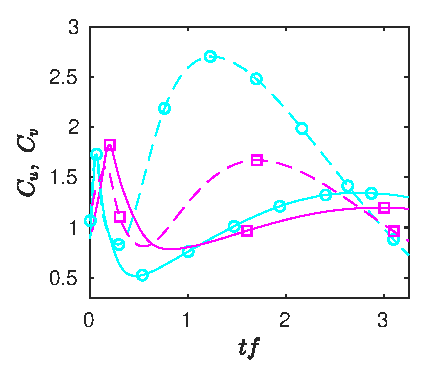
\includegraphics[width=2.85in,height=2in]{Cu_CV_combined}}
		%\put(-0.1,2.5){$\mathbf{(a)}$}
		%\put(1.2,0.01){\colorbox{white}{\makebox(0.75,0.15){}}}
	  \end{picture}
	\end{minipage}%
	\begin{minipage}{0.5\textwidth}
	\setlength{\unitlength}{1in}
	\begin{picture}(2.9,2)
		\put(0,0){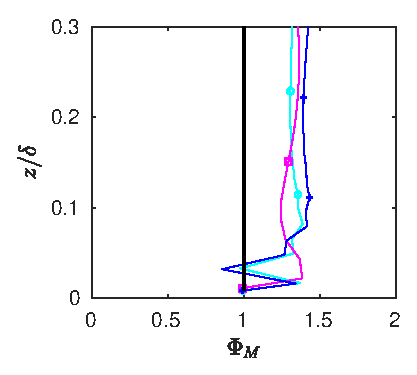
\includegraphics[width=2.85in,height=1.95in]{combined_phiM}}
		%\put(-0.1,2.5){$\mathbf{(b)}$}
		%\thicklines
        %\put(2.85,0.53){\line(0,1){1.42}}
	\end{picture}
	\end{minipage}
\caption{(a). $C_u, C_v$ plotted against non-dimensional time $tf$ for  EK10 ($-\circ-$) and EK02 ($-\square-$). Solid lines correspond to $C_u$ and dotted lines to $C_v$. (b). Nondimensional vertical gradient of mean streamwise velocity, $\Phi_M=\kappa z u_*^{-1} d\left < \bar{u} \right >/dz$ plotted as a function of nondimensional height for EK10 ($-\circ-$), EK02 ($-\square-$), CHNL ($-+-$). The solid black line corresponds to the classical log law expected to hold in the surface layer.}
\label{fig:cu-cv-phi_m}
\end{figure}
\noindent For a horizontally homogeneous turbulent flow field it can be shown that $C_u$ and $C_v$ will have a value of unity in steady state \citep{book-garrat-blm} condition. Unsteadiness in $C_u$ and $C_v$ with respect to the non-dimensional inertial time $tf$are shown in Fig.  \ref{fig:cu-cv-phi_m}$(a)$. Increased non-stationarity is observed in $EK10$ compared to $EK02$ although the oscillations in these cases tend to have similar time periods. The oscillations are expected to diminish  exponentially around the  $C_{u},\ C_{v}=1$ line \citep{book-garrat-blm} and the figure indicates that the simulations are reasonably converged. 

The nondimensional streamwise velocity gradient, $\Phi_M=\kappa z u_*^{-1} d\left < \bar{u} \right >/dz$ plotted against nondimensional height is shown in \ref{fig:cu-cv-phi_m}(b), where, $u_*= -(\left < (\bar{u}_{1}'\bar{u}_{3}'+\tau_{13,s})^2 + ( \bar{u}_{2}'\bar{u}_{3}'+ \tau_{23,s})^2\right >)^{1/4}$. Following similarity theory, $\Phi_M$ can be predicted to have a value of unity in the lowest $10\%$ of the boundary layer \citep{stoll_blm_2006}. The values obtained from the simulations are consistent across the different levels of rotation and similar to values obtained previously using LES \citep{stoll_blm_2006,andren_brown_qjrm_94}. 

In figure \ref{fig:uw-vw} normalized shear stresses are plotted and a difference between all the cases are apparent. In a horizontally homogeneous field under quasi-steady condition, the applied streamwise pressure gradient is expected to balance the total vertical stress gradient as evident from equation \ref{eqn:les_eqn}. As a result a linear vertical profile of total stress ($\left <\bar{u_1}'\bar{u_3}'+\tau_{13} \right>$)  is expected for the $CHNL$ case that goes from a normalized values of $-1$ to a value of zero at the domain top as shown in Fig. \ref{fig:uw-vw}$(a)$. For the $EK02$ and $EK10$ cases, a linear profile in ($\left <\bar{u}_{1}'\bar{u}_{3}'+\tau_{13} \right>$) does not emerge in these cases because of significant contribution to the stress profile from  the spanwise stress component($\left <\bar{u}_{2}'\bar{u}_{3}'+\tau_{23} \right>$) component that accounts for as much as $30\%$ at the ground level (Fig. \ref{fig:uw-vw}$(b)$). Figure \ref{fig:rossbyno} shows the difference in rotational tendencies between $EK10$ and $EK02$ in terms of the vertical profile of the local Rossby number defined as $Ro_{z} = \sqrt{\left <  \omega_{z}^2\right >}/f$ where, $\omega_z$ denotes the wall-normal component of the vorticity vector. With increasing height from the ground, the influence of the Coriolis grows larger which is manifested in a decreasing ratio of inertia to Coriolis forces. $EK02$ clearly shows a greater degree of influence of Coriolis force at every height compared to $EK10$. 
\graphicspath{{chap1Img/}}
\begin{figure}[htb]
	\begin{minipage}{0.5\textwidth}
	\setlength{\unitlength}{1in}
	  \begin{picture}(2.9,2)
		\put(0,0){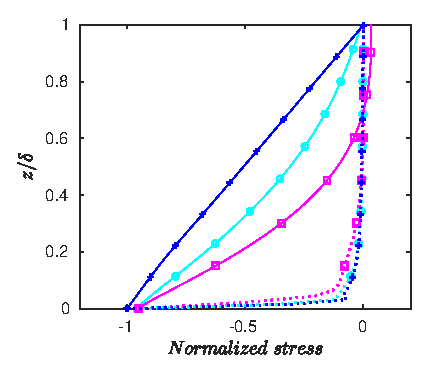
\includegraphics[width=2.85in,height=2in]{totalVerticalStress_uw_combined}}
		 \put(0.75,1.78){$(a)$}
		%\put(-0.1,2.5){$\mathbf{(a)}$}
		%\put(1.1,0.01){\colorbox{white}{\makebox(1.55,0.175){ $ \mathbf{({u'_{1}u'_{3}+ \tau_{13})}/u_*^{2}}$}}}		
		\thicklines
		%\put(2.844,0.47){\line(0,1){1.45}}
	  \end{picture}
	\end{minipage}%
	\begin{minipage}{0.5\textwidth}
	\setlength{\unitlength}{1in}
	\begin{picture}(2.9,2)
		\put(0,0){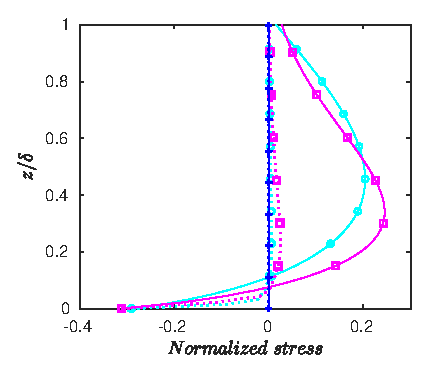
\includegraphics[width=2.85in,height=2in]{totalVerticalStress_vw_combined}}
		 \put(0.75,1.78){$(b)$}
		%\put(-0.1,2.5){$\mathbf{(b)}$}
		%\put(1.0,0.0){\colorbox{white}{\makebox(1.55,0.175){$ \mathbf{Normalized\ stress}$}}}
		\thicklines
     %   \put(2.85,0.47){\line(0,1){1.42}}
	\end{picture}
	\end{minipage}
\caption{Normalized vertical profiles of time and horizontally averaged resolved and SGS stresses. (a) $\left <\bar{u}'\bar{w}'+ \tau_{uw}\right>$ and $\tau_{uw}$ plotted as a function of height normalized by boundary layer height ($\delta$) for cases EK10 ($\circ$), EK02 ($\square$) and $CHNL$ (+). Solid lines correspond to $\left <\bar{u}'\bar{w}' + \tau_{uw} \right >$ and dotted lines correspond to $\tau_{uw}$. (b) $\left <\bar{v}'\bar{w}'+ \tau_{vw}\right>$ and $\tau_{vw}$ plotted as a function of normalized height for cases EK10 ($\circ$), EK02 ($\square$) and $CHNL$ (+). Solid lines correspond to $\left <\bar{v}'\bar{w}' + \tau_{vw} \right >$ and dotted lines to $\tau_{vw}$.}
\label{fig:uw-vw}
\end{figure}
\graphicspath{{chap1Img/}}
\begin{figure}
\setlength{\unitlength}{1in}
\begin{picture}(5,2)
\put(1,0){\includegraphics[width=2.85in,height=2in]{rossbyNo}}{}%
\end{picture}
\caption{Vertical Rossby number profile of $EK10$ and $EK02$ plotted as a function of normalized height.}
\label{fig:rossbyno}
\end{figure}

%\begin{table}[htb]
%\centering
%\caption{Simulation parameters and flow characteristics}
%\begin{tabular}{ c c c c c c c c c c c c}
%\hline 
% & Nx & Ny & Nz & $L_x$(Km) & $L_y$(Km) & $L_z$ (Km) & $U_g$ (m/s) & $u_*$ (m/s) & $\delta$(m) & $Ro$ & $f(s^{-1})$ \\
%\hline 
%$EK10$ & 2048 & 2048 & 64 & 120 & 120 & 1.5 & 10  & 0.41 & 1433.00  & 67 & 10$^{-4}$  \\
%$EK02$ & 2048 & 2048 & 64 & 120 & 120 & 0.75 & 2 & 0.09 & 550.69 & 33 & 10$^{-4}$ \\
%$CHNL$ & 2048 & 2048 & 64 & 120 & 120 & 1.5 & 0 & 0.42  & 1500.00 & - & - \\
%\hline 
%\hline 
%\end{tabular}
%\label{tab:sim_param}
%\end{table}

\begin{table}[ht]
\caption{Simulation parameters and flow characteristics}
  \begin{tabular}{ c c c  c c c c  c }
  \hline 
   & Nx/Ny & Nz & $L_x/L_y$(Km) & $L_z$ (Km) & $U_g$ (m/s)  & $\delta$(m) & $Ro$ \\
  \hline  
   $CHNL$ & 2048 &  64 & 128 &  1.5 & 0   & 1500.00 & - \\
   $EK10$ & 2048 &  64 & 128 &  1.5 & 2   & 1433.00 & 67  \\
   $EK02$ & 2048 &  64 & 128 &  0.75 & 2  & 550.69 & 33  \\
  \hline 
  \hline 
\end{tabular}
\label{tab:sim_param}
\end{table}
\subsection{Autocorrelation and spectral characteristics}
The resolved velocity fields contain a  range of large active length scales that are similar or greater to the boundary layer height \citep{}. One common method to estimate the extent of the large active scales in the flow is using the autocorrelation function. One of the primary uses for the autocorrelation function is to define an integral length scale for a flow and although, by definition VLSMs are larger than the integral length scale,  autocorrelation function still provides a relative measure of flow length scales in the three different cases analyzed ( Fig. \ref{fig:corr}). The panels on the left hand side of figure \ref{fig:corr} show the streamwise velocity correlation of the mid-boundary layer plane ( $z_{ref}=\delta/2$ ) with all other discrete horizontal levels (i.e. $ 0.015\delta, 0.031\delta, 0.047\delta, 0.063\delta, 0.079\delta$) that were resolved in the simulation. The formal definition of this correlation is 
\begin{align}
 R_{uu}^{3d}(\Delta x, \Delta y, & z, z_{ref})   =   \frac{\left < u'(x, y, z_{ref})u'(x+ \Delta x, y + \Delta y, z) \right >}{\left < u'^{2}(x,y,z_{ref})\right >} \ ,
\label{eqn:3d_corr} 
\end{align}
where, $\Delta x, \Delta y$ are spatial lags between the two points in streamwise and spanwise directions, respectively. Typically,  juxtaposed low- and high-momentum streaks  in the spanwise direction have been identified as a signature of the existence of VLSMs. For the $CHNL$ case, iso-surfaces of both positive and negative correlation are visible where $R_{uu}^{3d}\geq 0.25$ is denoted by the red iso-surfaces and $R_{uu}^{3d}\leq -0.15$ is denoted by blue iso-surfaces. The $EK10$ and $EK02$ cases do not show negative iso-surfaces on either of the sides of the positively correlated regions. This is a  first sign of the impact of rotation on characteristics of VLSMs. These plots also show the maximum vertical extent of influence of active scales existing in the mid-boundary layer. In $CHNL$, the influence of the largest active scales extends from the bottom of the domain up to   $85\%$ of the BL height. This was limited to $80\%$ for the $EK10$ and $70\%$ for the $EK02$ cases.  The panels on the right hand side of Fig. \ref{fig:corr} show planar autocorrelation of $u_1$-velocity component at $ z=0.25\delta$ where, the planar autocorrelation is defined as: 
\begin{align}
 R_{uu}^{2d}(\Delta x, \Delta y, z)=\frac{\left < u'(x, y, z)u'(x+ \Delta x, y + \Delta y, z) \right >}{\left < u'^{2}(x,y,z)\right >} \ .
 \label{eqn:2d_corr}
\end{align}
Shape, orientation and spread of the iso-lines are noticeably different for the three cases. Iso-lines of nominal correlation of 0.01 along with -0.1, 0.1, 0.25 are shown. Regions of negative correlation displayed by black lines most prominently appear in  the $CHNL$ case. For the $EK10$ case very small regions of negative correlation are visible and for the $EK02$ case negligibly small regions of negative correlation  appear alongside of large elongated positively correlated regions. The rotated orientation of the iso-lines in $EK10$ and $EK02$ are indicative of the presence of rotation in the flows while the iso-lines are almost aligned with $x$ and $y$ axes in $CHNL$  suggesting  a mean streamwise flow. A greater degree of rotation in the counter-clockwise direction in $EK02$ compared to $EK10$ is also apparent from the orientation of the iso-lines corresponding to $0.1$ and $0.25$.  
%----------------------------------autocorrelation plot---------------------------------- -------
\graphicspath{{chap1Img/}}
\begin{figure}
\centering {
	\begin{minipage}{0.49\textwidth}
	  \setlength{\unitlength}{1in}
	  \begin{picture}(3,2.5)
		  \put(0,0.0){{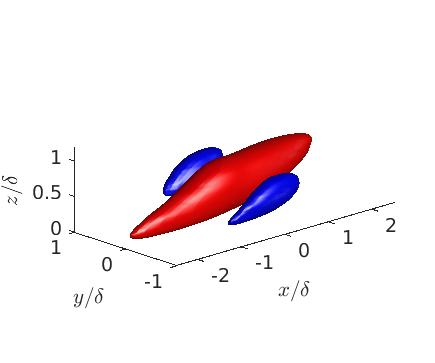
\includegraphics[width=3.0in,height=2.5in]{corr3d-with-midBL-chnl}}}{}% 
		  \put(0.75,1.78){$(a)$}
		\end{picture}
	\end{minipage}%
	\begin{minipage}{0.49\textwidth}
	\setlength{\unitlength}{1in}
	    \begin{picture}(3,2.5)
		    \put(0,0){{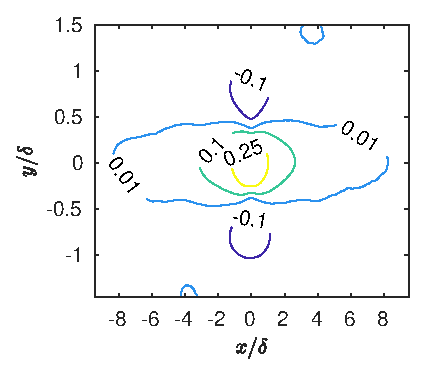
\includegraphics[width=2.5in,height=2in]{corr2d_z_delta_0d47_chnl}}}{}% 
		    \put(0.75,1.78){$(a')$}
		  \end{picture}
	\end{minipage}%	
	
	\begin{minipage}{0.49\textwidth}
	\setlength{\unitlength}{1in}
	  \begin{picture}(3,2.5)
		  \put(0,0){{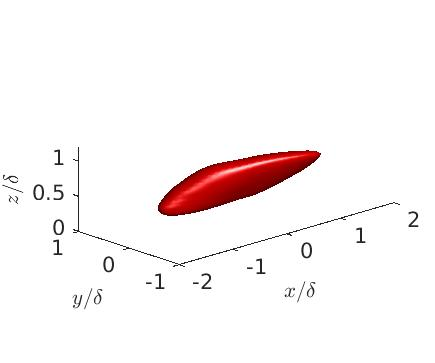
\includegraphics[width=3.0in,height=2.5in]{corr3d-with-midBL-ug10}}}{}% 
		  \put(0.75,1.78){$(b)$}
		\end{picture}
  \end{minipage}
  	\begin{minipage}{0.49\textwidth}
  	\setlength{\unitlength}{1in}
	  \begin{picture}(3,2.5)
		  \put(0,0){{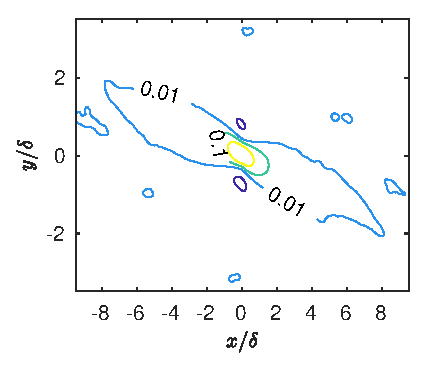
\includegraphics[width=2.5in,height=2in]{corr2d_z_delta_0d47_ek10}}}{}% 
		  \put(0.75,1.78){$(b')$}
		\end{picture}
  \end{minipage}	
  
	\begin{minipage}{0.49\textwidth}
	\setlength{\unitlength}{1in}
	  \begin{picture}(3,2.5)
		  \put(0,0){{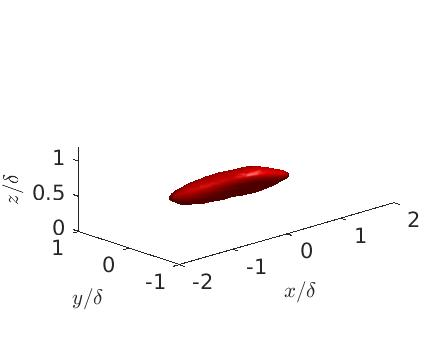
\includegraphics[width=3.0in,height=2.5in]{corr3d-with-midBL-ug02}}}{}% 
		  \put(0.75,1.78){$(c)$}
		\end{picture}
  \end{minipage}
  	\begin{minipage}{0.49\textwidth}
  	\setlength{\unitlength}{1in}
	  \begin{picture}(3,2.5)
		  \put(0,0){{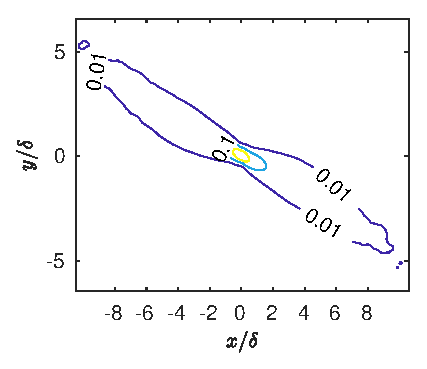
\includegraphics[width=2.5in,height=2in]{corr2d_z_delta_0d47_ek02}}}{}% 
		  \put(0.75,1.78){$(c')$}
		\end{picture}
  \end{minipage}  
}
\caption{Correlation of u-velocity component. $(a)$, $(b)$, $(c)$ show correlation of reference level $z/\delta=0.5$ with all other horizontal levels as defined by equation \ref{eqn:3d_corr} for $CHNL$, $EK10$, and $EK02$, respectively. Red iso-surfaces denote correlation greater than or equal to $0.25$ and blue iso-surfaces show negative correlation, smaller or equal to $-0.15$.  $(a', b', c')$. Show planar autocorrelation, $R_{uu}^{2D}$ of $CHNL$, $EK10$, and $EK02$ at $z=0.5\delta$, respectively.}
\label{fig:corr}
\end{figure}
\graphicspath{{chap1Img/}} 
\begin{figure}
\begin{minipage}{0.5\textwidth}%
  \setlength{\unitlength}{1in}
  \begin{picture}(2.9,2)
  \put(0,0){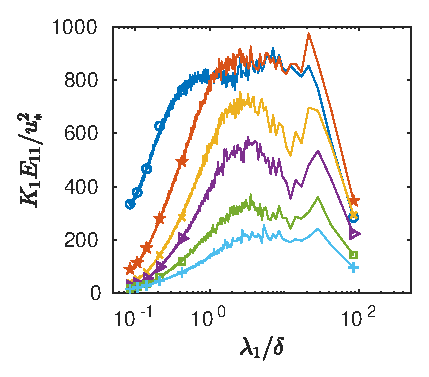
\includegraphics[width=2.85in,height=2in]{premult_u_spec_stream-wise-frame_chnl}}
  \put(0.76,1.7){$(a)$}
  \end{picture}%
\end{minipage}
\begin{minipage}{0.49\textwidth}%
  \setlength{\unitlength}{1in}
  \begin{picture}(2.9,2)
  \put(0,0){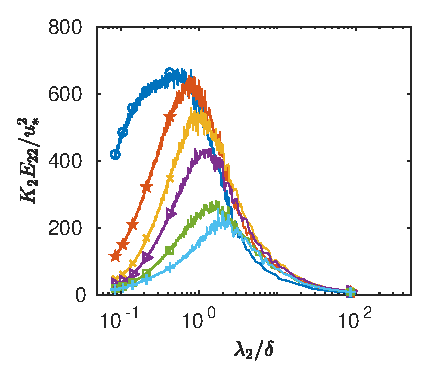
\includegraphics[width=2.85in,height=2in]{premult_v_spec_span-wise-frame_chnl}}
  \put(0.76,1.7){$(a')$}
  \end{picture}
\end{minipage}

\begin{minipage}{0.5\textwidth}%
  \setlength{\unitlength}{1in}
  \begin{picture}(2.9,2)
  \put(0,0){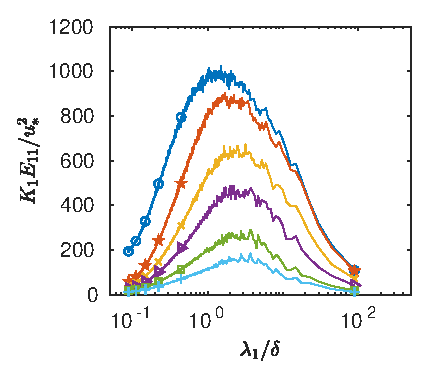
\includegraphics[width=2.85in,height=2in]{premult_u_spec_stream-wise-frame_ug10}}
  \put(0.76,1.7){$(b)$}
  \end{picture}
\end{minipage}%
\begin{minipage}{0.49\textwidth}
   \setlength{\unitlength}{1in}
  \begin{picture}(2.9,2)
  \put(0,0){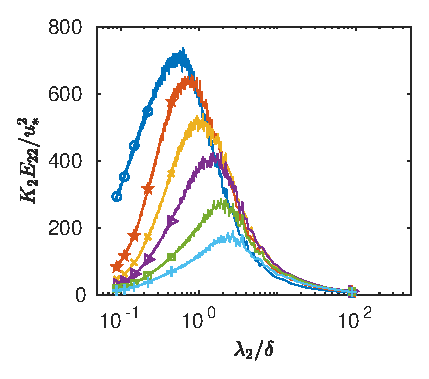
\includegraphics[width=2.85in,height=2in]{premult_v_spec_span-wise-frame_ug10}}
  \put(0.76,1.7){$(b')$}
  \end{picture}
\end{minipage}

\begin{minipage}{0.5\textwidth}%
  \setlength{\unitlength}{1in}
  \begin{picture}(2.9,2)
  \put(0,0){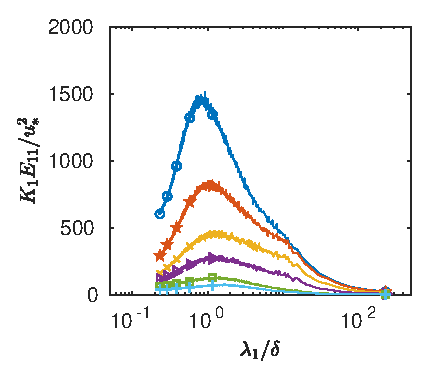
\includegraphics[width=2.85in,height=2in]{premult_u_spec_stream-wise-frame_ug2}}
  \put(0.76,1.7){$(c)$}
  \end{picture}
\end{minipage}%
\begin{minipage}{0.49\textwidth}%
   \setlength{\unitlength}{1in}
  \begin{picture}(2.9,2)
  \put(0,0){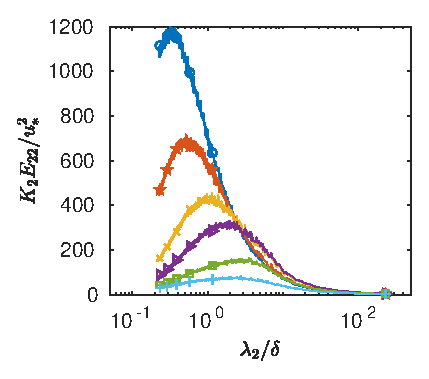
\includegraphics[width=2.85in,height=2in]{premult_v_spec_span-wise-frame_ug2}}
  \put(0.76,1.7){$(c')$}
  \end{picture}
\end{minipage}

\caption{Premultiplied velocity spectra against normalized wavelengths are shown for different cases. $(a)$, $(b)$, $(c)$ show spectra of the $u$-component of the velocity for $CHNL$, $EK10$ and $EK02$, respectively. $(a')$, $(b')$ and $(c')$ show spectra of the $v$-component of the velocity for $CHNL$, $EK10$ and $EK02$, respectively. Curves marked with ($\smallcircle, \smallwhitestar, \times, {\smalltriangleup}, \smwhtsquare, \plus$) correspond to heights $z/\delta = (0.06,\ 0.15, \ 0.30,\ 0.45, \ 0.71, \ 0.90)\pm 0.01$, respectively.}
\label{spec_pre_spec}
 \end{figure}
From the lines marked by nominal positive correlation of $0.01$ it can be inferred that the unidirectional pressure gradient in channel flow helps retain high coherence of the velocity field and the rotation in geostrophic flows substantially prohibits this coherence. This assessment can be quantified by the examination of integral length scales which can be defined in streamwise and cross-stream directions as $L_{int,x}=\int_0^{\infty} dx\ R_{uu}^{2d}(x,0)$ and $L_{int,y}=\int_0^{\infty} dy\ R_{uu}^{2d}(0,y)$, respectively. Here, a discrete version of the integral length scales were used following \citep{traumner_blm_2015} where, $\Delta x_o$ and $\Delta y_0$ indicate the location of zero crossings of the correlation function on the x and y axes, respectively. 
\begin{align}
L_{int,x}=\sum_{\Delta x=0}^{\Delta x_{0}}R_{uu}^{2d}(x+\Delta x, 0,z)\Delta x \ \text{and}
\label{eqn:L_x}
\end{align}

\begin{align}
L_{int,y}=\sum_{\Delta y=0}^{\Delta y_{0}}R_{uu}^{2d}(0, y+\Delta y,z)\Delta y\ .
\label{eqn:L_y}
\end{align}
Equations \ref{eqn:L_x} and \ref{eqn:L_y} were evaluated at $z=0.25\delta$. Streamwise integral length scale of $CHNL$ was determined  to be $2569\ m$ and that of $EK10$ and $EK02$ were, respectively, $877\ m$ and $265\ m$. Cross-stream integral length scales were, respectively, $382\ m$, $300\ m$ and $160\ m$ for the three cases. 

The high energy peak in the  long wavelength region or a plateau region in the longer wavelengths regime in the pre-multiplied spectra has primarily been the source of identification of VLSMs in channel flows \citep{guala_adrian_jfm2006, fang2015blm}. In figure \ref{spec_pre_spec} the pre-multiplied spectra of the velocity components are presented. The spectra is  premultiplied by wavenumber and normalized by friction velocity and the $x$-axes wavelength is normalized by $\delta$.  In the $CHNL$ case (fig. \ref{spec_pre_spec}a), the typical high energy peak and plateau region in the long wavelength regime can be identified, confirming the existence of the streamwise aligned large scale structures along with VLSMs. The first peak or the beginning of the plateau, corresponds to LSMs and the second peak or the end of the plateau corresponds to VLSMs. This plateau region with a slope of zero also corresponds to the $-1$ slope region of traditional Fourier spectra where inertial range scales are usually identified with a matching $-5/3$ slope \citep{perry_chng_jfm_86,saddoughi1994}. In this case of premultiplied spectra the area under any curve corresponds to the total turbulent energy due to the streamwise velocity at a particular distance from the wall. The same common trend of decrease in turbulent energy with respect to distance from the wall is evident for all cases. It is noticeable in $CHNL$  that for a height of $0.06\delta$ the peak appears at the wavelength of $18\delta$ whereas, at the height of $0.47\delta$ the peak appears at $10\delta$. In general a monotonic trend of reduction in range of the wavelength of the active energy producing scales is evident in $CHNL$. High energy peaks corresponding to VLSMs shift towards smaller wavelength region with an overall shrinking plateau region as the distance from the wall increases with a notable exception of $z=0.11\delta$. This exception was also found in a similar LES study \citep{fang2015blm}.  Also, as the height increases the distinctive peak in the LSM region corresponding to a large amount of energy gradually ceases to exist. This indicates that in the lower portion of the BL, LSMs contribute significantly to the total energy content.   All these features conform to the findings of the previous studies that probed  VLSM characteristics in channel flows. However, in the case of Ekman layer flows denoted by subfigures ($b$) and ($c$)  significantly  different energy distributions are observed. Instead of bi-modal, skewed mono-modal distributions with or without a clear plateau region are produced. For the $CHNL$ and $EK10$ cases the highest energy peaks in the LSM regime shift towards the larger wavelengths with increasing distance from the wall. In contrast, for the $EK02$ case the shift toward  larger wavelengths is not as prominent and all of the peaks are concentrated near $\lambda_x/\delta=1$. The observed difference in the length scales of the high energy containing motions between the Ekman layer cases i.e. $EK10$ and $EK02$ can be attributed to the difference in the magnitude of rotation present in the flows. Also, the spectral energy distributions in $EK02$  are flatter than those of the EK10 case while at the same time the relative energy content of LSMs diminishes significantly. This could either mean the absence of VLSMs or that their contribution to the stream-wise energy is not as pronounced as in the other cases. The tails of the spectral energy distributions show significant difference between the three cases. The $CHNL$ case has a sharp fall in the energy content of the small scale structures, while $EK10$ has  a gradual decline and $EK02$ has a even slower decline. 

On the right hand side panels  ($a'$), ( $b'$), and ($c'$) show pre-multiplied and normalized $u_2$-spectra with respect to spanwise wavelengths normalized by $\delta$. The possibility  of streamwise aligned large-scale structures  being washed out due to the cross-stream velocity component can be inferred from $u_2$-spectra. Intense energy in the cross stream scales would indicate such a possibility. The energy  distributions in the cross-stream scales in these cases are mono-modal with or without a clear plateau. The energy distributions the cross-stream velocity scales are similar between the different cases unlike the $u_1$-spectra. The high-energy peaks move towards the larger wavelength region with increasing distance from the wall. $CHNL$ and $EK10$  show nearly similar distribution each with its most significant large scale being on the order of $\delta$. At similar heights,  similar length scales tend to have more energy in $EK10$ compared to $CHNL$. This is due to a higher magnitude in fluctuations of the $u_2$ velocity component. Energy content at each scale at each horizontal level is lower in $EK02$ compared to $EK10$ with a notable exception at $z= 0.054\delta$. These pre-multiplied spectra do not provide any conclusive evidence of the absence of VLSMs in Ekman layer  flows although they do not show any evidence of the presence either.  To address this issue in the next section alternative approaches are used to identify VLSMs that involve selective filtering and alternative VLSM definitions as well as quantifying the contributions of VLSMs to the surface shear stress.


\noindent  

\begin{table*}[!htb]
%\scriptsize
\centering
\caption{Percentage cumulative energy of all the scales greater than the specified threshold at $z=0.47\delta$ (approx.)}
\begin{tabular*}{0.9\textwidth}{ c@{\hskip 0.35in} c@{\hskip 0.35in} c@{\hskip 0.35in} c@{\hskip 0.35in} c@{\hskip 0.35in} c@{\hskip 0.35in} c@{\hskip 0.3in} c@{\hskip 0.3in} }
\hline
\hline
 Threshold & $\delta$ & $2\delta$ & $3\delta$ & $4\delta$ & $5\delta$ & $6\delta$  & $7\delta$  \\ % & $8\delta$  \\
\hline 
$CHNL$ & 0.811 & 0.674 & 0.581 & 0.515 & 0.464 & 0.423 &  0.391  \\ %& 0.366 \\
$EK10$ & 0.757 & 0.584 & 0.479 & 0.402 & 0.348 & 0.304 & 0.271   \\ %& 0.244  \\
$EK02$ & 0.679 & 0.486 & 0.384 & 0.319 & 0.273 & 0.239 & 0.212   \\ %& 0.190  \\
%\hline 
%\hline 
\end{tabular*}
\label{tab:prcnt_cum_energy}
%\end{table}
%
%\begin{table*}[!htb]
\begin{tabular*}{0.9\textwidth}{c@{\hskip 0.35in} c@{\hskip 0.35in} c@{\hskip 0.35in} c@{\hskip 0.35in} c@{\hskip 0.350in} c@{\hskip 0.350in}  c@{\hskip 0.35in} c}
\hline

 Threshold & $9\delta$& $10\delta$ & $11\delta$ & $12\delta$ & $14\delta$ & $16\delta$ & $18\delta$ \\
\hline 
$CHNL$ & 0.345 & 0.327 & 0.310 & 0.291 & 0.264 & 0.242 & 0.222 \\
$EK10$ & 0.220 & 0.199 & 0.183  & 0.171 & 0.151 & 0.133 & 0.117 \\
$EK02$ & 0.171 & 0.154 & 0.140 & 0.128 & 0.108 & 0.093 & 0.080 \\
\hline 
\hline 
\end{tabular*}
%\label{tab:prcnt_cum_energy}
\end{table*}

\subsection{Filtering and Conditional Averaging}
Conditional averaging was carried out with a goal of further characterizing the size and shape of VLSMs and of identifying the contribution of VLSMs to shear stress, $\tau_{x,y} = \sqrt((u_{1}'u_{3}')^2+(u_{2}'u_{3}')^2)$, where, $u_{1}'u_{2}'= (u_{1} -\left< u_{1}\right >_{x,y})(u_{2} -\left< u_{2}\right >_{x,y})$, and $u_{2}'u_{3}'= (u_2 -\left< u_{2}\right >_{x,y})(u_{3} -\left< u_{3}\right >_{x,y})$ with $\left < \right >_{x,y}$ denoting the planar average. The conditional averaging was carried out at selected wall parallel planes to characterize the flows in the wall-normal direction and to have a quantitative account the of coherent structures on horizontal planes. Many studies have examined  the characteristics and contributions of coherent structures with length scales of order of $\delta$ or smaller \citep{}. Here, to facilitate the determination of contributions from only large scale coherent structures, smaller flow scales that  fall within the inertial sub-range of turbulence were removed by filtering.  Two-dimensional spectral cut-off filtering in the horizontal plane was used and the cut-off scale was selected as the distance of the selected surface from the ground. This filtering was designed to remove all horizontal scales smaller than the scales  of the energy producing eddies.  A new alternative definition of planar coherent structures was adopted to facilitate our analysis. Two-dimensional coherent structures were defined as the connected region of pixels either having negative $u_{1}'$ fluctuations (low momentum) or positive $u_{1}'$ fluctuations (high momentum). The adopted definition was motivated by the commonly reported presence of VLSMs in filtered velocity fields identified through visualization \citep{hutchins_marusic_jfm2007,dennis_nickels_jfm2011}.  Visually, VLSMs appear to be long regions of low or high momentum fitting the definition assumed.  Here, an objective analysis was devised using image-processing techniques to detect such long structures and quantify their spatial characteristics. In addition, to quantify the importance of a detected structure to momentum transport the ratio of shear stress fraction and area fraction was determined.  

Here, horizontal transects of 3D structures were identified at different heights. To identify a 2D horizontal-transect of a structure a binary version of the velocity field was created. To identify low-momentum structures all positive streamwise velocity field fluctuations were set to zero and negative values were assigned a value of one so that on a given horizontal level 

\begin{equation}
	u_{1}'(x,y) = \begin{cases}	
	1, &\text{$u_{1}' \leq 0$ }\\
	0, &\text{$u_{1}' >  0$}\ .
	\end{cases}
	\label{case:binary-vel}
\end{equation}
\noindent Next the binary planar image was segmented and labeled using a connected component labeling technique \cite{book_comp_vision_davies}. Spatial image moments and shape attributes for each labeled area were calculated including the centroid, area, major axis length, minor axis length, and orientation. The zeroth-order moment of a shape is the area of that shape. The ratio of first-order and zeroth-order moments yields the centroid of an image object. The major axis length is equivalent of the major axis length of an ellipse that has the same moments of inertia along the horizontal and vertical axes and also has the same moments of inertia along the principal axes. The orientation was measured as degrees of angle between the horizontal axis and the major axis of a shape.  More details on spatial moments and discrete binary image shape attributes can be found in \citet{book_intro_dimg_proc_pratt}. The major axis length of each labelled segment was and if it was greater than a specified threshold, the segment was marked as a possible horizontal transect through a VLSM. On these marked image objects ellipses with pre-determined major and minor axes lengths were drawn with coincident centroids. All such elliptical areas in five statistically independent frames were then averaged to characterize an  average footprint of a VLSM. The frames were $L_{int,x}/U_c$ (sec) apart from each other in time where, the characteristic velocity $U_c$ was taken as the mean velocity at the height of the BL.  In the image segment identification process, an incremental range of length scales $(0.75n-1.25n)\delta $ with $n= 2,3,.\ .\  .\  . \ 24$ was used.  Structures identified with in each  range of scales on selected horizontal levels provided cumulative measurements of the contribution to the shear stress and turbulent kinetic energy by coherent structures on those 2D planes.

To quantify the importance and contribution of VLSMs to shear stress two quantities were calculated after averaging, the area fraction and the shear stress fraction. The total area fraction $A_f$, was calculated as, 
\begin{equation*}
		A_f = \sum \frac{\mathbb{N}}{\mathbb{N}_a},
\label{eqn:area_frac_def}        
\end{equation*}
\noindent where $\mathbb{N}$ represents the number of non-zero pixels  within an individual ellipse and $\mathbb{N}_a$ denotes the total number of pixels in the binary image. Summation over all area fractions yielded total area fraction. The total shear stress fraction $\tau_{x,y}^f$ was  calculated as, 
\begin{equation*}
		\tau_{x,y}^f =\frac{\sum \left < \tau_{x,y} \right > \mathbb{N}}{\left < \tau_{x,y}\right >_a\mathbb{N}_a },
\label{eqn:stress_frac_def}             
\end{equation*}
\noindent where $\left < \tau_{x,y}\right >_a$  is the average shear stress of the wall parallel plane and $\left < \tau_{x,y} \right >$ is that of a selected elliptical area.  An example of the determination process is presented in Fig. \ref{area_binarized_vel_image}. The image on the left hand side shows  a binarized image of the $u_{1}'$ field at the height of $0.15\delta$.  The white regions represent negative $u_{1}'$ fluctuations and black regions represent positive velocity regions. In this picture all detected structures having  lengths in the range  of $\delta-10\delta$ are shown as blue regions. On the right hand side, a two blue regions  encircled with red  ellipses and marked interior points painted in blue are shown.  The detected regions were characterized with the major and minor axes lengths of the bounding ellipses and the painted blue points were used as sampling points for calculating average shear stress. Finally, the ratio $\tau_{x,y}^f/A_f$ was studied to quantify the significance of the selected areas in terms of  their contribution towards the shear stress.  
% for two column wide figures use figure*
\graphicspath{{chap1Img/}}
\begin{figure}[htb]
	\begin{minipage}{0.5\textwidth}
	\setlength{\unitlength}{1in}
	  \begin{picture}(2.9,2)
		\put(0,0){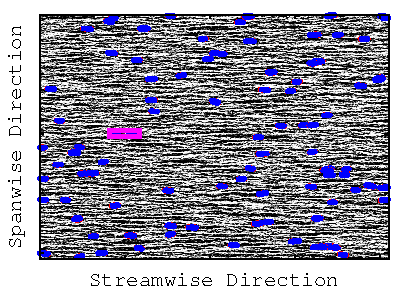
\includegraphics[width=2.85in,height=2in]{chnl_bin_lowMom-eps-converted-to}}
		%\put(-0.1,2.5){$\mathbf{(a)}$}
		\put(0.5,-0.01){\colorbox{white}{\makebox(1.9,0.175){ $ {Streamwise\ direction}$ }}}	
		\put(-0.15,-0.1){\colorbox{white}{\makebox(0.25,2.175){\rotatebox{90}{$ {Spanwise\ direction}$}}}}	
	  \end{picture}
	\end{minipage}%
	\begin{minipage}{0.5\textwidth}
	\setlength{\unitlength}{1in}
	\begin{picture}(2.9,2)
		\put(0,0){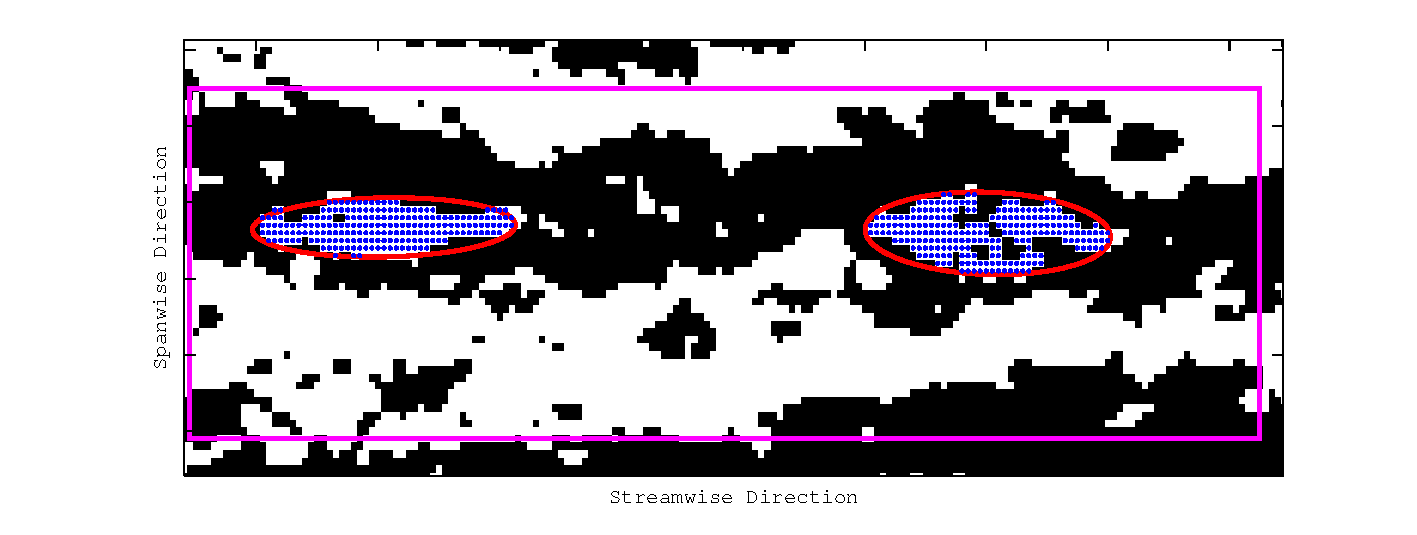
\includegraphics[width=2.85in,height=2.05in]{cropped-eps-converted-to}}
		\put(0.5,-0.01){\colorbox{white}{\makebox(1.9,0.175){ $ {Streamwise\ direction}$ }}}	
		\put(-0.0005,-0.1){\colorbox{white}{\makebox(0.25,2.175){\rotatebox{90}{${Spanwise\ direction}$}}}}		
	\end{picture}
	\end{minipage}
\caption{(Left) For the $CHNL$ case a cropped binarized negative $u'$ velocity field image is shown which is overlayed with detected elliptical coherent structures with a range of major axis length lengths, $\delta-10\delta$. (Right) Zoomed-in two detected structures with interior points painted in blue where average shear stresses were calculated are shown. Horizontal and vertical axes are aligned with streamwise and spanwise directions respectively} 
\label{area_binarized_vel_image}
\end{figure}
\graphicspath{{chap1Img/}}
\begin{figure}
\centering {
	\begin{minipage}{0.49\textwidth}
	  \setlength{\unitlength}{1in}
	  \begin{picture}(2.9,2.08)
		  \put(0,0){{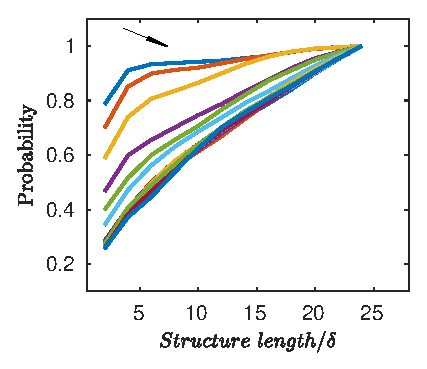
\includegraphics[width=2.65in,height=2in]{struclen_cdf_chnl}}}{}% 
		  \put(2.2,0.55){$(a)$}
		\end{picture}
	\end{minipage}%
	\begin{minipage}{0.49\textwidth}
	\setlength{\unitlength}{1in}
	    \begin{picture}(2.9,2.08)
		    \put(0,0){{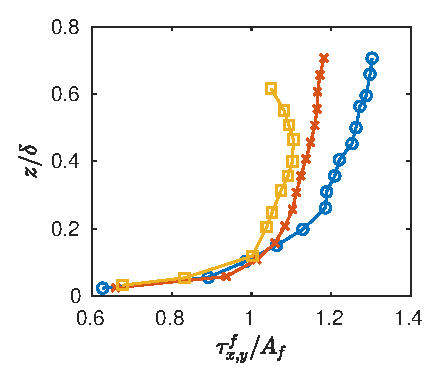
\includegraphics[width=2.85in,height=2.06in]{flux_area_frac_ratio_all_band}}}{}% 
		    \put(2.2,0.55){$(d)$}
		  \end{picture}
	\end{minipage}%	
	
	\begin{minipage}{0.49\textwidth}
	\setlength{\unitlength}{1in}
	  \begin{picture}(2.9,2.08)
		  \put(0,0){{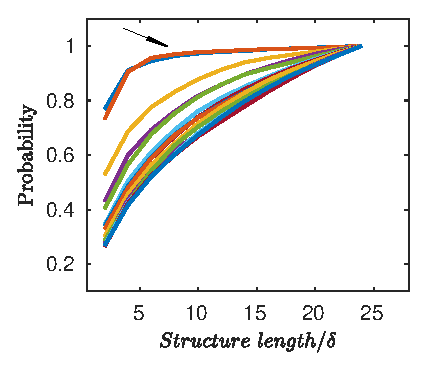
\includegraphics[width=2.65in,height=2in]{struclen_cdf_ek10}}}{}% 
		  \put(2.2,0.55){$(b)$}
		\end{picture}
  \end{minipage}
  	\begin{minipage}{0.49\textwidth}
  	\setlength{\unitlength}{1in}
	  \begin{picture}(2.9,2.08)
		  \put(0,0){{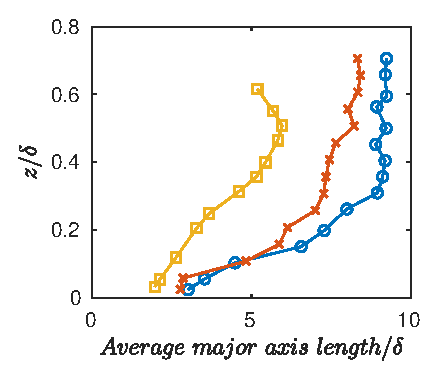
\includegraphics[width=2.85in,height=2.06in]{avg_majorAxisLength_all_band}}}{}% 
		  \put(2.2,0.55){$(e)$}
		\end{picture}
  \end{minipage}	
  
	\begin{minipage}{0.49\textwidth}
	\setlength{\unitlength}{1in}
	  \begin{picture}(2.9,2.08)
		  \put(0,0){{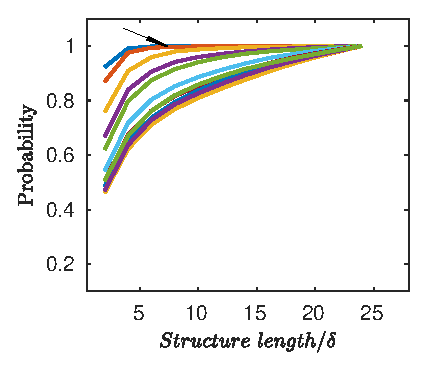
\includegraphics[width=2.65in,height=2in]{struclen_cdf_ek02}}}{}% 
		  \put(2.2,0.55){$(c)$}
		\end{picture}
  \end{minipage}
  	\begin{minipage}{0.49\textwidth}
  	\setlength{\unitlength}{1in}
	  \begin{picture}(2.9,2.08)
		  \put(0,0){{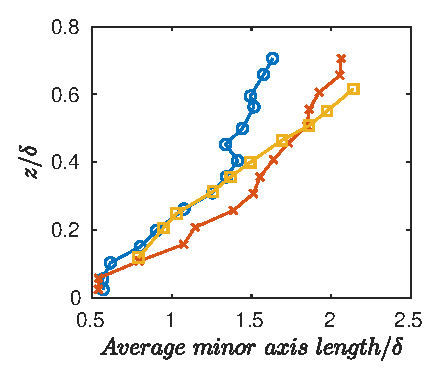
\includegraphics[width=2.85in,height=2.06in]{avg_minorAxisLength_all_band}}}{}% 
		  \put(2.2,0.55){$(f)$}
		\end{picture}
  \end{minipage}  
}
\caption{Cumulative density function of coherent structure lengths, their aggregate contribution to shear stress as functions of height and their average lengths. The left panel shows cumulative density function of the structure lengths detected in the range $\delta-25\delta$ for $CHNL$ (a), $EK10$ (b), and $EK02$ (c) cases. The arrows point to the direction of increasing distance from the surface. The panel on the right hand side shows the ratio (d) $\tau_{x,y}^f/A_f$ plotted for different wall normal locations of all cases. (e) shows the mean length of major axes for all structures detected  and (f) shows the mean minor axes lengths. Here ($\circ$) represents $CHNL$, ($\times$) represents $EK$10, and ($\Box$) represents $EK02$.}
\label{fig:stress_cont_cdf_length}
\end{figure} 
Fig. \ref{fig:stress_cont_cdf_length}  shows cumulative density functions of the lengths of coherent structures as a function of height in the left panels along with the ratio  $\tau_{x,y}^f/A_f$ in the right  panels. The cumulative density functions highlight differences in the population of VLSMs existing  in the $u_1$-velocity fields. Between the three cases $CHNL$ shows the presence of VLSM horizontal transects  as large as $30\delta$ on a surface-parallel plane at the height of  $0.66\delta$ and similar observation can  for $EK10$ and $EK02$. However,  a comparison of figures \ref{fig:stress_cont_cdf_length}(a), (b) and (c) indicates that ratio of large-scale structures to small scale structures decreases for higher degrees of rotation  in the velocity field. Also evident is the fact that the large-scale structures are scarce at lower levels i.e. in the surface layer but appear more frequently as the distance from the ground increases  i.e. outer layers. In general the number of occurrences of large-scale structures is a function of height.  To get a quantitative picture of the importance of such detected structures to horizontal shear stress, $\tau_{x,y}^f/A_f$ is plotted against normalized height in Fig. \ref{fig:stress_cont_cdf_length}(d).  Due to huge differences in the number of detected structures in each band, $\tau_{x,y}^f/A_f$ in Fig. \ref{fig:stress_cont_cdf_length}(d), average major axis length in \ref{fig:stress_cont_cdf_length}(e), and average minor axis length in \ref{fig:stress_cont_cdf_length}(f) at each horizontal level were calculated as the expected values. 
%The weights were determined as $N_{band}/\sum N_{band}$, where,  $N_{band}$ represents the number of detected structures in each band such as the number of structures having lengths within the band $(0.75*18-1.25*18)\delta$, following the band definition  $(0.75n-1.25n)\delta $; where  $n= 2,3,.\ .\  .\  . \ 24$. 
The $\tau_{x,y}^f/A_f$ ratio plot shows the importance of the structures detected in terms of their contribution to over all shear stress at the respective horizontal levels.  $CHNL$  shows the highest  contribution to shear stress from  connected regions  while $EK02$ shows  the minimum contribution.  This figure also reveals a significant fact that structures or at least the VLSM horizontal transects on surface-parallel planes  do not contribute significantly to shear stress in the surface layer.  However, the authors refrain from drawing any strong conclusion from this result in the vicinity of the surface because of the use of a highly approximate modeled shear stress boundary condition in LES of the ABL.  In general, as the distance from the bottom surface increases, the importance and contribution of these visually-identified long connected regions of low momentum increases gradually. The length scale of VLSMs likewise can also be observed to be a function of $z$ in figure \ref{fig:stress_cont_cdf_length}(e). Although, a slight difference in the maximum average  length of the structures is observed in $CHNL$ and $EK10$ cases i.e. $8.19\delta$ at a height of $0.7\delta$ for $CHNL$ case and $8.4\delta$ at a height of $0.65\delta$ for $EK10$ (fig. \ref{fig:stress_cont_cdf_length}(e)), the trend in these two cases are almost identical. The shortest among the maximum average length appears in $Ek02$  as $5.95\delta$ at a height of $0.5\delta$.  As evident from the Fig. \ref{fig:stress_cont_cdf_length}(f), the structure width increases with height consistently.  At the highest measurement height $CHNL$  shows the minimum structure width i.e. $1.47\delta$ whereas, $EK10$ and $EK02$  show $2.06\delta$ and $2.13\delta$, respectively. With the introduction of rotation in the velocity field the structures become shorter but wider. 

A visual depiction of the 3D structure of the reported VLSMs as connected regions of low momentum fluid is shown in fig. \ref{fig:vlsm-3d}. To determine the 3D structure the binarized $u_{1}'$ velocity field was examined for 2D horizontal transects on the horizontal plane at $2\Delta_z$ distance away from the ground where, $\Delta_z$ is the vertical grid spacing of the staggered grid. Upon identification of any connected region having a major axis length longer than a specified threshold, an enclosing 3D box was drawn centered at the centroid of the region. The 3D rectangular box extended from the bottom wall to the top of the simulation domain. The horizontal dimensions of the box in the streamwise and spanwise directions for the three different cases were estimated from the corresponding expected dimensions of the VLSMs (fig. \ref{fig:stress_cont_cdf_length}(d) and \ref{fig:stress_cont_cdf_length}(e)). The horizontal box dimensions were large enough to contain the VLSMs within the box and had streamwise lengths of $15\delta$, $15\delta$, $10\delta$ and constant spanwise length of $2\delta$ for $CHNL$, $EK10$ and $EK02$, respectively.  The conditional averaging revealed the average 3D shape of a VLSM which is expected from the very nature of the operation of conditional averaging. The fact that should be emphasized here is that the detection-condition was imposed only on a horizontal plane and no constraint was in place to the 3D shape or orientation. The assumption of similarity in size, orientation and shape of the structures around the selected averaging points is inherent to the idea of conditional averaging. If the assumptions hold true then a 3D coherent shape would appear.  Considering these facts it can be inferred that the 3D structures obtained reveals a few characters of the VLSM.  The conspicuous differences between VLSMs identified in each case appear in shape and dimension. For the $CHNL$ case on an average VLSMs appear to have a symmetrical cylindrical shape in the middle which gets tapered off near the ends and the length in the mean wind direction is approximately $9\delta$. $Ek10$ case shows a structure which is slightly shorter in the mean wind direction and shows signs of rotation near the top where $Ro$ is relatively low compared to that near the surface (see fig. \ref{fig:rossbyno}). The average length can be identified to be approximately $7\delta$. For the $EK02$ case a much shorter but wider structure is obtained. The effect of rotation in this case is the most prominent. The length can be identified to be approximately $5.7\delta$. 

\graphicspath{{chap1Img/}}
\begin{figure}
\centering {
	\begin{minipage}{0.49\textwidth}
	  \setlength{\unitlength}{1in}
	  \begin{picture}(2.9,2)
		  \put(0,0){{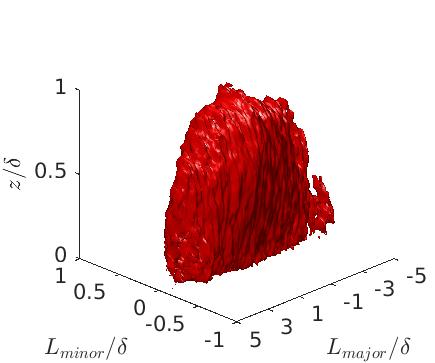
\includegraphics[width=2.89in,height=2in]{vlsm_chnl}}}{}% 
		  \put(0.75,1.5){$(a)$}
		\end{picture}
	\end{minipage}%
	\begin{minipage}{0.48\textwidth}
    	\setlength{\unitlength}{1in}
	    \begin{picture}(2.9,2)
		    \put(0,0){{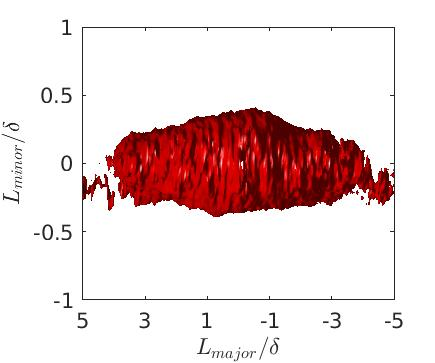
\includegraphics[width=2.89in,height=2in]{vlsm_chnl_topView}}}{}% 
		    \put(0.75,1.5){$(a')$}
		  \end{picture}
	\end{minipage}%	
	
	\begin{minipage}{0.49\textwidth}
	 \setlength{\unitlength}{1in}
	  \begin{picture}(2.9,2)
		  \put(0,0){{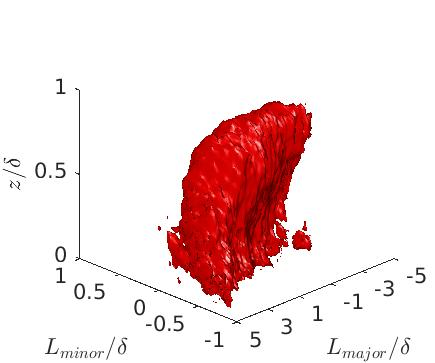
\includegraphics[width=2.89in,height=2in]{vlsm_ek10}}}{}% 
		  \put(0.75,1.5){$(b)$}
		\end{picture}
  \end{minipage}
  	\begin{minipage}{0.49\textwidth}
  	\setlength{\unitlength}{1in}
	  \begin{picture}(2.9,2)
		  \put(0,0){{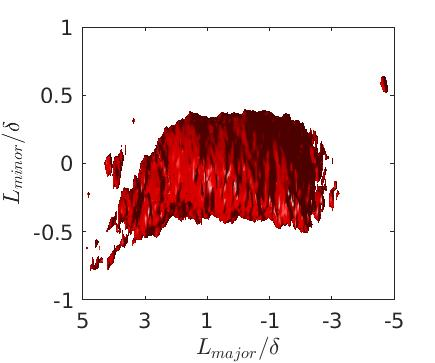
\includegraphics[width=2.89in,height=2in]{vlsm_ek10_topView}}}{}% 
		  \put(0.75,1.5){$(b')$}
		\end{picture}
  \end{minipage}	
  
	\begin{minipage}{0.49\textwidth}
	\setlength{\unitlength}{1in}
	  \begin{picture}(2.9,2)
		  \put(0,0){{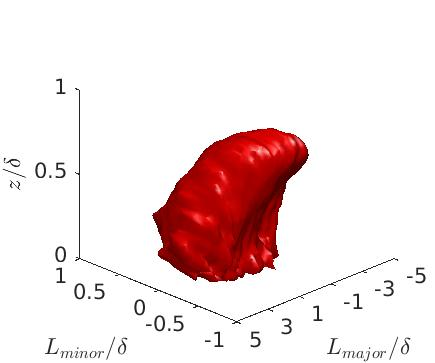
\includegraphics[width=2.89in,height=2in]{vlsm_ek02}}}{}% 
		  \put(.75,1.5){$(c)$}
		\end{picture}
  \end{minipage}
  	\begin{minipage}{0.49\textwidth}
  	\setlength{\unitlength}{1in}
	  \begin{picture}(2.9,2)
		  \put(0,0){{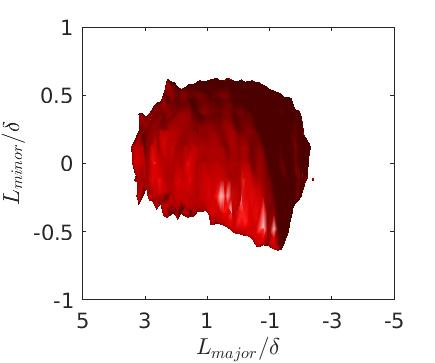
\includegraphics[width=2.89in,height=2in]{vlsm_ek02_topView}}}{}% 
		  \put(0.75,1.5){$(c')$}
		\end{picture}
  \end{minipage}  
}
\caption{$(a)$, $(b)$, $(c)$ show the average 3D structures projected from detected 2D transects at the height of the first vertical grid point for the $CHNL$, $EK10$ and $EK02$ cases, respectively. $(a')$, $(b')$, $(c')$ show the top view of the same 3D structures as shown on the left panels. Iso surfaces enclose values less than $\left < u\right >-1.5\sigma_{u}$ }
\label{fig:vlsm-3d}
\end{figure} 
% BibTeX users please use one of
\graphicspath{{chap1Img/}}
%\begin{figure}
%\centering
%{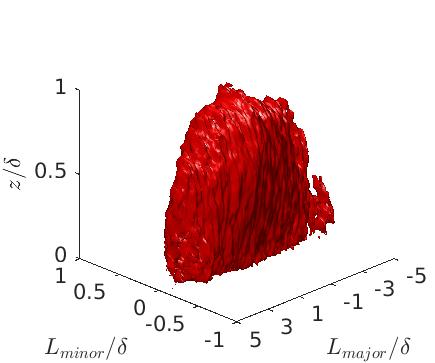
\includegraphics[width=4.5in,height=3.0in]{vlsm_chnl}}{}%
%\hspace{1cm}%
%{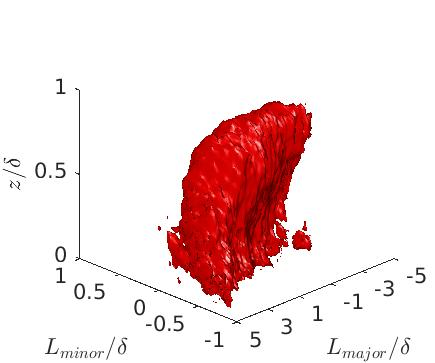
\includegraphics[width=4.5in,height=3.0in]{vlsm_ek10}}{}
%\hspace{1cm}%
%{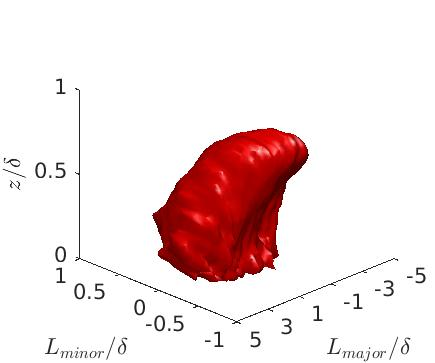
\includegraphics[width=4.5in,height=3.0in]{vlsm_ek02}}{}{} 
%\caption{Averaged velocity field based on low momentum  trigger. On top the velocity field is shown for $CHNL$ and on the middle and bottom $Ek10$ and $EK02$, respectively. Lengths of structures along the major axis , minor axis, and wall-normal directions are normalized by boundary layer depth ($\delta$). Iso-surfaces enclose  points in the  averaged field having a $u'$ value less than $\left < u' \right >-1.5\sigma_{u'}$. $\sigma$ is the standard deviation of the entire $u'$velocity field. }
%\label{fig:vlsm-3d}
%\end{figure}

\section{Conclusion}
VLSMs were identified and their relative scales were compared for three different simulated flows. The simulation domain was large enough compared to the length scale of VLSMs not to impose any inhibition in the spatial development of these structures. One simulation provided the canonical channel flow case and the other two were Ekman layer simulations characterized by different degrees of rotation. Differences in the flow cases in terms of basic turbulent statistics along with the coherence were discussed. Coherence in the flows were compared in the light of correlation between different horizontal planes and integral length scales. The unidirectional constant pressure driven flow was observed to have the highest degree of coherence. The differences in coherence among the flow cases are reflected in the the determined mean length scales of the composite 3D structures of VLSMs.

Previously, VLSMs were reported for flows only where rotation did not have any significant effect. Thus, the challenges of identification of VLSMs in rotational flows were not addressed. The most common problem in identification and detection of VLSMs is the lack of a concrete definition based upon which a detection algorithm could be developed. To address this issue and to test a hypothesis that VLSMs could be identified based on the reported visual characteristics of those structures i.e. as long streaks of low momentum fluid primarily elongated in the streamwise direction, an alternative simple definition of VLSM was adopted. VLSMs were defined as the long connected regions of low momentum fluid. This definition yielded quantitatively consistent length scales of VLSMs with the same detected from pre-multiplied spectra for the $CHNL$. The detection of length scales of VLSMs from one dimensional pre-multiplied spectra quickly becomes marred as soon as rotation is introduced in the flow since, distinguishable dominant peaks ceases to appear. Adopting the alternative definition and utilizing the established image processing techniques lend to an effective technique of detection and measurement that work well even when rotation is introduced in the flow. This was verified by the identification of VLSMs in Ekman layer flows. A simple linear correspondence of the streamwise length scale was not observed with local Rossby number however, it was observed that in general rotation inhibits the streamwise length scale of the VLSMs but is conducive to the increase in length scale in the cross-stream direction. The greater the influence of rotation compared to inertial acceleration, the greater the cross-stream length scale is. It was also observed that irrespective of the forcing condition the length scale of the two dimensional planar structures were increasing in the direction normal to the ground. This result is consistent with the findings of \citet{de_silva_hutchins_jfm_2016}. 

\bibliographystyle{plainnat}
\bibliography{MyThesisRefs}
\end{document}
